\chapter{System Architecture and Design}


This chapter presents the overall system architecture, module design, SQLite relational database schema, sequence diagrams, state machine diagram, AI and voice interaction architecture, and privacy/security design for \textbf{Bear Buddy}. All technical decisions in this chapter are aligned with the requirements in Chapter 3, the story interaction model in Chapter 4, and the UI-UX specifications in Chapter 5.


\section{Architectural Overview and Technology Stack}



\subsection{Offline-First and Mode-Separated Architecture}


Bear Buddy adopts a \textbf{Modular Offline-First Client Architecture} structured around the \textbf{MVVM (Model – View – ViewModel)} pattern on mobile devices. This architecture directly addresses the core constraints of the domain:

\begin{enumerate}
  \item \textbf{Zero Network Dependency for the Child Learning Flow (\texttt{FR22}, \texttt{NFR12})}: All bundled/downloaded social stories, visual illustrations, narration controllers, and the SQLite database reside locally on the device. A child (\texttt{PERS01}) can complete stories reliably at home or in a classroom without internet connectivity.
  \item \textbf{Strict Isolation between Child Mode and Caregiver Mode (\texttt{DD31}, \texttt{DD32})}: The application state coordinator (\texttt{AppStore} / \texttt{SessionCoordinator}) segregates the child view hierarchy (\texttt{S08}–\texttt{S14}, \texttt{S24}) from the caregiver management hierarchy (\texttt{S01}–\texttt{S07}, \texttt{S15}–\texttt{S23}) behind the \texttt{CaregiverAuthGuard} verification boundary.
  \item \textbf{Fault-Isolated AI and Speech Adapters}: External AI story recommendation and on-device Scenario E speech recognition are encapsulated behind adapter interfaces with strict timeouts and deterministic local fallbacks, guaranteeing that service failures never block or interrupt a child's story session (\texttt{NFR13}, \texttt{DD36}, \texttt{DD40}).
\end{enumerate}



\begin{figure}[htbp]
\centering
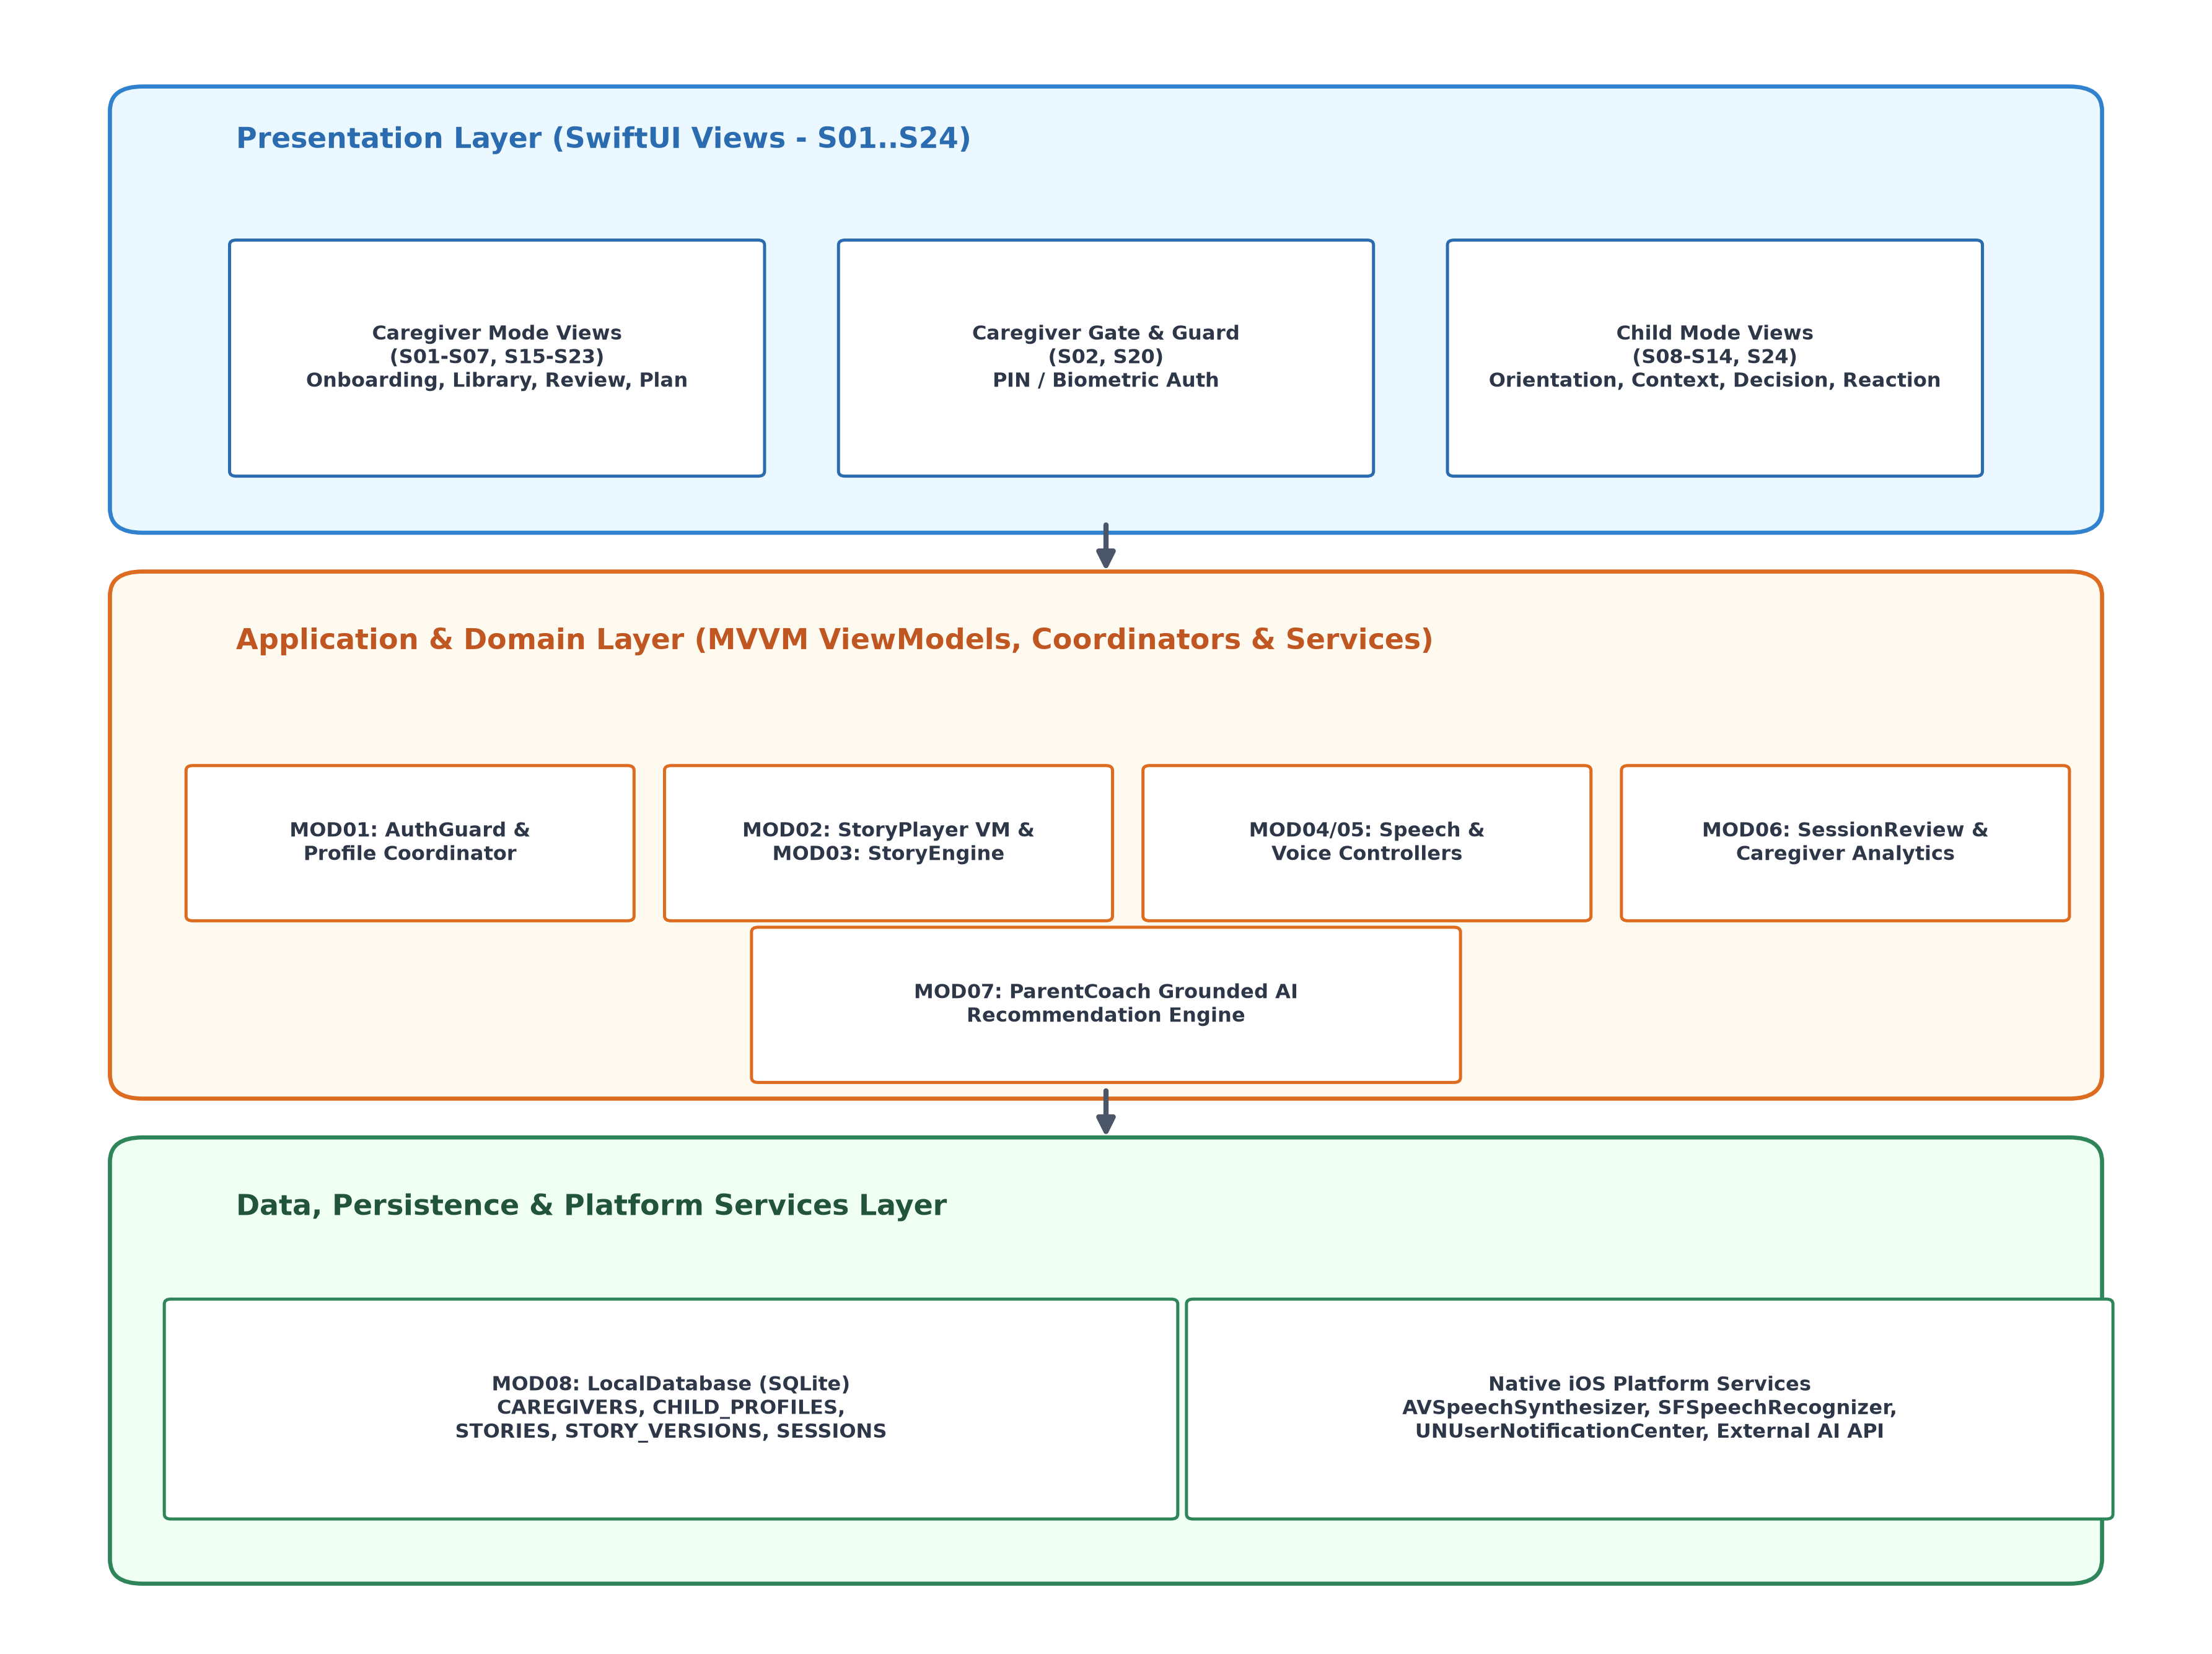
\includegraphics[width=0.95\textwidth]{figures/system_architecture.png}
\caption{Three-Layer Offline-First and Mode-Separated System Architecture}
\label{fig:system_architecture}
\end{figure}



\subsection{Technology Choices and Cross-Device Data Strategy}


\noindent\begin{xltabular}{\textwidth}{|p{3.2cm}|p{4.0cm}|X|}
\hline
\textbf{Architectural Layer} & \textbf{Selected Technology} & \textbf{Rationale and Alignment with Bear Buddy Requirements} \\ \hline
\endhead
\textbf{Mobile Platform \& UI Framework} & \textbf{iOS / iPadOS 17.0+} with \textbf{SwiftUI} & Declarative reactive UI with native support for Dynamic Type ($200\%$ font scaling), VoiceOver, Reduce Motion, and precise hit-target sizing (\texttt{NFR01}–\texttt{NFR07}). \\ \hline
\textbf{Frontend Architecture} & \textbf{MVVM (Model – View – ViewModel)} & Decouples the interactive story state machine (\texttt{Understand} $\rightarrow$ \texttt{Predict} $\rightarrow$ \texttt{Choose} $\rightarrow$ \texttt{Observe} $\rightarrow$ \texttt{Why} $\rightarrow$ \texttt{Repeat}) from SwiftUI views, enabling deterministic unit testing of story branches and system states (\texttt{S23}). \\ \hline
\textbf{Local Relational Database} & \textbf{SQLite3} (\texttt{LocalDatabase}) & Lightweight, ACID-compliant relational storage with foreign-key enforcement; supports structured multi-version story storage (\texttt{story\_version}), role-based access links, and granular interaction logs without requiring a mandatory backend server. \\ \hline
\textbf{Cross-Device Data Exchange Strategy} & \textbf{Local SQLite + Controlled Encrypted Sync/Export Package} & Addresses the architectural note in Section 1.4.2: SQLite serves as the primary local source of truth; when a parent (\texttt{PERS02}) links a profile with a support teacher (\texttt{PERS03}), only the authorized child profile and versioned session logs are synchronized/exported within the explicitly granted scope. \\ \hline
\textbf{Audio Narration \& Speech Recognition} & \textbf{AVFoundation (\texttt{AVSpeechSynthesizer})} \& \textbf{Speech (\texttt{SFSpeechRecognizer})} & Enables single-stream audio queue management to prevent overlapping narration (\texttt{DD23}), adjustable Vietnamese speech rates, and on-device keyword recognition for Scenario E. \\ \hline
\textbf{Local Activity Reminders} & \textbf{UserNotifications (\texttt{UNUserNotificationCenter})} & Schedules caregiver activity reminders locally on the device without relying on third-party push notification servers. \\ \hline
\end{xltabular}



\section{Module Design and Complete Traceability Matrix}



\subsection{Module Responsibilities}


The system is decomposed into 8 cohesive modules (\texttt{MOD01}–\texttt{MOD08}):

\begin{itemize}
  \item \textbf{\texttt{MOD01} — Account, Profile \& Role Guard Module (\texttt{ProfileModels}, \texttt{CaregiverGate})}: Manages caregiver authentication, child profile CRUD, role-based access control between Parent (\texttt{PERS02}) and Support Teacher (\texttt{PERS03}), and privacy consent audit logging (\texttt{consent\_audit\_logs}).
  \item \textbf{\texttt{MOD02} — Versioned Story Library Module (\texttt{StoryRepository}, \texttt{StoryModels})}: Manages story retrieval across the 4 situational categories (\texttt{CAT01}–\texttt{CAT04}), keyword/filter queries, transparent popularity metrics, and immutable \texttt{story\_version} resolution.
  \item \textbf{\texttt{MOD03} — Interactive Story Engine Module (\texttt{StoryPlayerViewModel})}: The core state machine governing \texttt{Child Mode} sessions, handling \texttt{Choice Card} and \texttt{Tap-to-Order} inputs, routing \texttt{Action} $\rightarrow$ \texttt{Reaction} $\rightarrow$ \texttt{Why} branches, and executing \texttt{Replay}, \texttt{Retry}, \texttt{Pause}, and \texttt{Need Help}.
  \item \textbf{\texttt{MOD04} — Accessibility \& Audio Narration Module (\texttt{SpeechController}, \texttt{AppColors})}: Applies per-profile font scaling, contrast tokens, and motion settings, and enforces single-stream narration playback so multiple taps never overlap audio.
  \item \textbf{\texttt{MOD05} — Scenario E Voice \& Touch Fallback Module (\texttt{VoiceInteractionController})}: Manages bounded short-phrase practice on \texttt{S24}, checks microphone permissions, performs keyword matching, and guarantees immediate touch-card fallback on error or refusal.
  \item \textbf{\texttt{MOD06} — Session Logger, Review \& Plan Module (\texttt{ParentViews}, \texttt{ReminderService})}: Records chronological child interaction events pinned to \texttt{story\_version}, renders descriptive \texttt{Session Review} screens (\texttt{S15}, \texttt{S16}), and manages \texttt{Learning Plans} and reminders (\texttt{S17}, \texttt{S19}).
  \item \textbf{\texttt{MOD07} — Explainable Parent AI Coach Module (\texttt{ParentCoachService})}: Combines local rule-based filtering with grounded AI queries to recommend library stories accompanied by human-readable match reasons (\texttt{S18}).
  \item \textbf{\texttt{MOD08} — Local Persistence \& System State Module (\texttt{LocalDatabase}, \texttt{AppStore})}: Provides transactional SQLite3 data access, manages the offline feedback queue (\texttt{S22}), and coordinates system/error states (\texttt{S23}).
\end{itemize}



\subsection{Complete Traceability Matrix}


Completing the requirement established in Section 5.7.3, the table below provides end-to-end traceability linking \textbf{User Needs (\texttt{UN}) $\rightarrow$ Requirements (\texttt{FR}/\texttt{NFR}) $\rightarrow$ Use Cases (\texttt{UC}) $\rightarrow$ UX Decisions (\texttt{DD}) $\rightarrow$ Screens (\texttt{S}) $\rightarrow$ Architecture Modules (\texttt{MOD})}:

\begin{footnotesize}
\noindent\begin{xltabular}{\textwidth}{|p{1.5cm}|p{2.2cm}|X|p{2.0cm}|p{2.0cm}|p{1.8cm}|}
\hline
\textbf{User Need (\texttt{UN})} & \textbf{Requirements (\texttt{FR} / \texttt{NFR})} & \textbf{Use Cases (\texttt{UC})} & \textbf{UX Decisions (\texttt{DD})} & \textbf{Screens (\texttt{S01}–\texttt{S24})} & \textbf{Architecture Modules (\texttt{MOD})} \\ \hline
\endhead
\textbf{UN01} (Understand context prior to choice) & \texttt{FR09}, \texttt{FR10} & \texttt{UC04}, \texttt{UC06} & \texttt{DD13}, \texttt{DD14} & \texttt{S07}, \texttt{S09} & \texttt{MOD02}, \texttt{MOD03} \\ \hline
\textbf{UN02} (Participate without independent reading) & \texttt{FR05}, \texttt{FR10}, \texttt{FR11}, \texttt{NFR01}, \texttt{NFR06} & \texttt{UC03}, \texttt{UC06} & \texttt{DD7}–\texttt{DD12}, \texttt{DD20} & \texttt{S04}, \texttt{S08}, \texttt{S09} & \texttt{MOD03}, \texttt{MOD04} \\ \hline
\textbf{UN03} (Clear orientation \& predictability) & \texttt{FR05}, \texttt{FR10}, \texttt{FR16}, \texttt{NFR09}, \texttt{NFR10} & \texttt{UC06}, \texttt{UC08} & \texttt{DD2}–\texttt{DD6} & \texttt{S08}–\texttt{S12}, \texttt{S14} & \texttt{MOD03} \\ \hline
\textbf{UN04} (Forgiving tap input \& non-mandatory voice) & \texttt{FR12}, \texttt{FR18}, \texttt{NFR03}, \texttt{NFR04}, \texttt{NFR06} & \texttt{UC07}, \texttt{UC10} & \texttt{DD26}–\texttt{DD30}, \texttt{DD36} & \texttt{S10}, \texttt{S24} & \texttt{MOD03}, \texttt{MOD05} \\ \hline
\textbf{UN05} (Understand Why, Replay \& Retry) & \texttt{FR13}, \texttt{FR14} & \texttt{UC08} & \texttt{DD15}–\texttt{DD19} & \texttt{S11}, \texttt{S12} & \texttt{MOD03}, \texttt{MOD06} \\ \hline
\textbf{UN06} (Sensory control \& self-paced learning) & \texttt{FR03}, \texttt{FR11}, \texttt{FR15}, \texttt{FR16}, \texttt{NFR05}, \texttt{NFR08} & \texttt{UC03}, \texttt{UC06}, \texttt{UC09} & \texttt{DD21}–\texttt{DD23}, \texttt{DD34}, \texttt{DD37} & \texttt{S04}, \texttt{S09}–\texttt{S14} & \texttt{MOD03}, \texttt{MOD04} \\ \hline
\textbf{UN07} (Caregiver library search \& story preview) & \texttt{FR01}, \texttt{FR06}–\texttt{FR09}, \texttt{FR21} & \texttt{UC01}, \texttt{UC04}, \texttt{UC12} & \texttt{DD31}, \texttt{DD32} & \texttt{S01}, \texttt{S05}–\texttt{S07}, \texttt{S17} & \texttt{MOD01}, \texttt{MOD02}, \texttt{MOD06} \\ \hline
\textbf{UN08} (Version-pinned \& profile-scoped review) & \texttt{FR02}–\texttt{FR04}, \texttt{FR19}–\texttt{FR22}, \texttt{NFR16} & \texttt{UC02}, \texttt{UC11}, \texttt{UC12} & \texttt{DD31}–\texttt{DD33}, \texttt{DD38} & \texttt{S02}, \texttt{S03}, \texttt{S15}, \texttt{S16} & \texttt{MOD01}, \texttt{MOD06}, \texttt{MOD08} \\ \hline
\textbf{UN09} (Explainable \& reviewable AI suggestions) & \texttt{FR17}, \texttt{FR18}, \texttt{NFR15} & \texttt{UC05}, \texttt{UC10} & \texttt{DD36}, \texttt{DD39} & \texttt{S18}, \texttt{S24} & \texttt{MOD05}, \texttt{MOD07} \\ \hline
\textbf{UN10} (Child agency to Pause or Ask for Help) & \texttt{FR15}, \texttt{NFR08} & \texttt{UC09} & \texttt{DD37} & \texttt{S08}–\texttt{S13} & \texttt{MOD03}, \texttt{MOD06} \\ \hline
\textbf{UN11} (Child data minimization \& access control) & \texttt{FR01}–\texttt{FR04}, \texttt{FR23}, \texttt{NFR14}, \texttt{NFR15} & \texttt{UC01}, \texttt{UC02}, \texttt{UC13} & \texttt{DD33}, \texttt{DD34}, \texttt{P11} & \texttt{S01}–\texttt{S03}, \texttt{S20} & \texttt{MOD01}, \texttt{MOD08} \\ \hline
\textbf{UN12} (Resilient error handling, Offline \& Support) & \texttt{FR18}, \texttt{FR22}, \texttt{FR24}, \texttt{FR25}, \texttt{NFR12}, \texttt{NFR13} & \texttt{UC04}, \texttt{UC05}, \texttt{UC10}, \texttt{UC14} & \texttt{DD24}, \texttt{DD40} & \texttt{S21}–\texttt{S24} & \texttt{MOD05}, \texttt{MOD07}, \texttt{MOD08} \\ \hline
\end{xltabular}
\end{footnotesize}



\section{SQLite Database Design}


The local SQLite database (\texttt{MOD08 - LocalDatabase}) is normalized to guarantee: (1) strict separation between caregiver accounts, child profiles, and revocable teacher access links; (2) immutable multi-version story storage (\texttt{story\_versions}) so historical session reviews remain accurate even after content updates; and (3) descriptive, non-punitive interaction logging.


\subsection{Entity-Relationship Diagram (ERD)}



\begin{figure}[htbp]
\centering
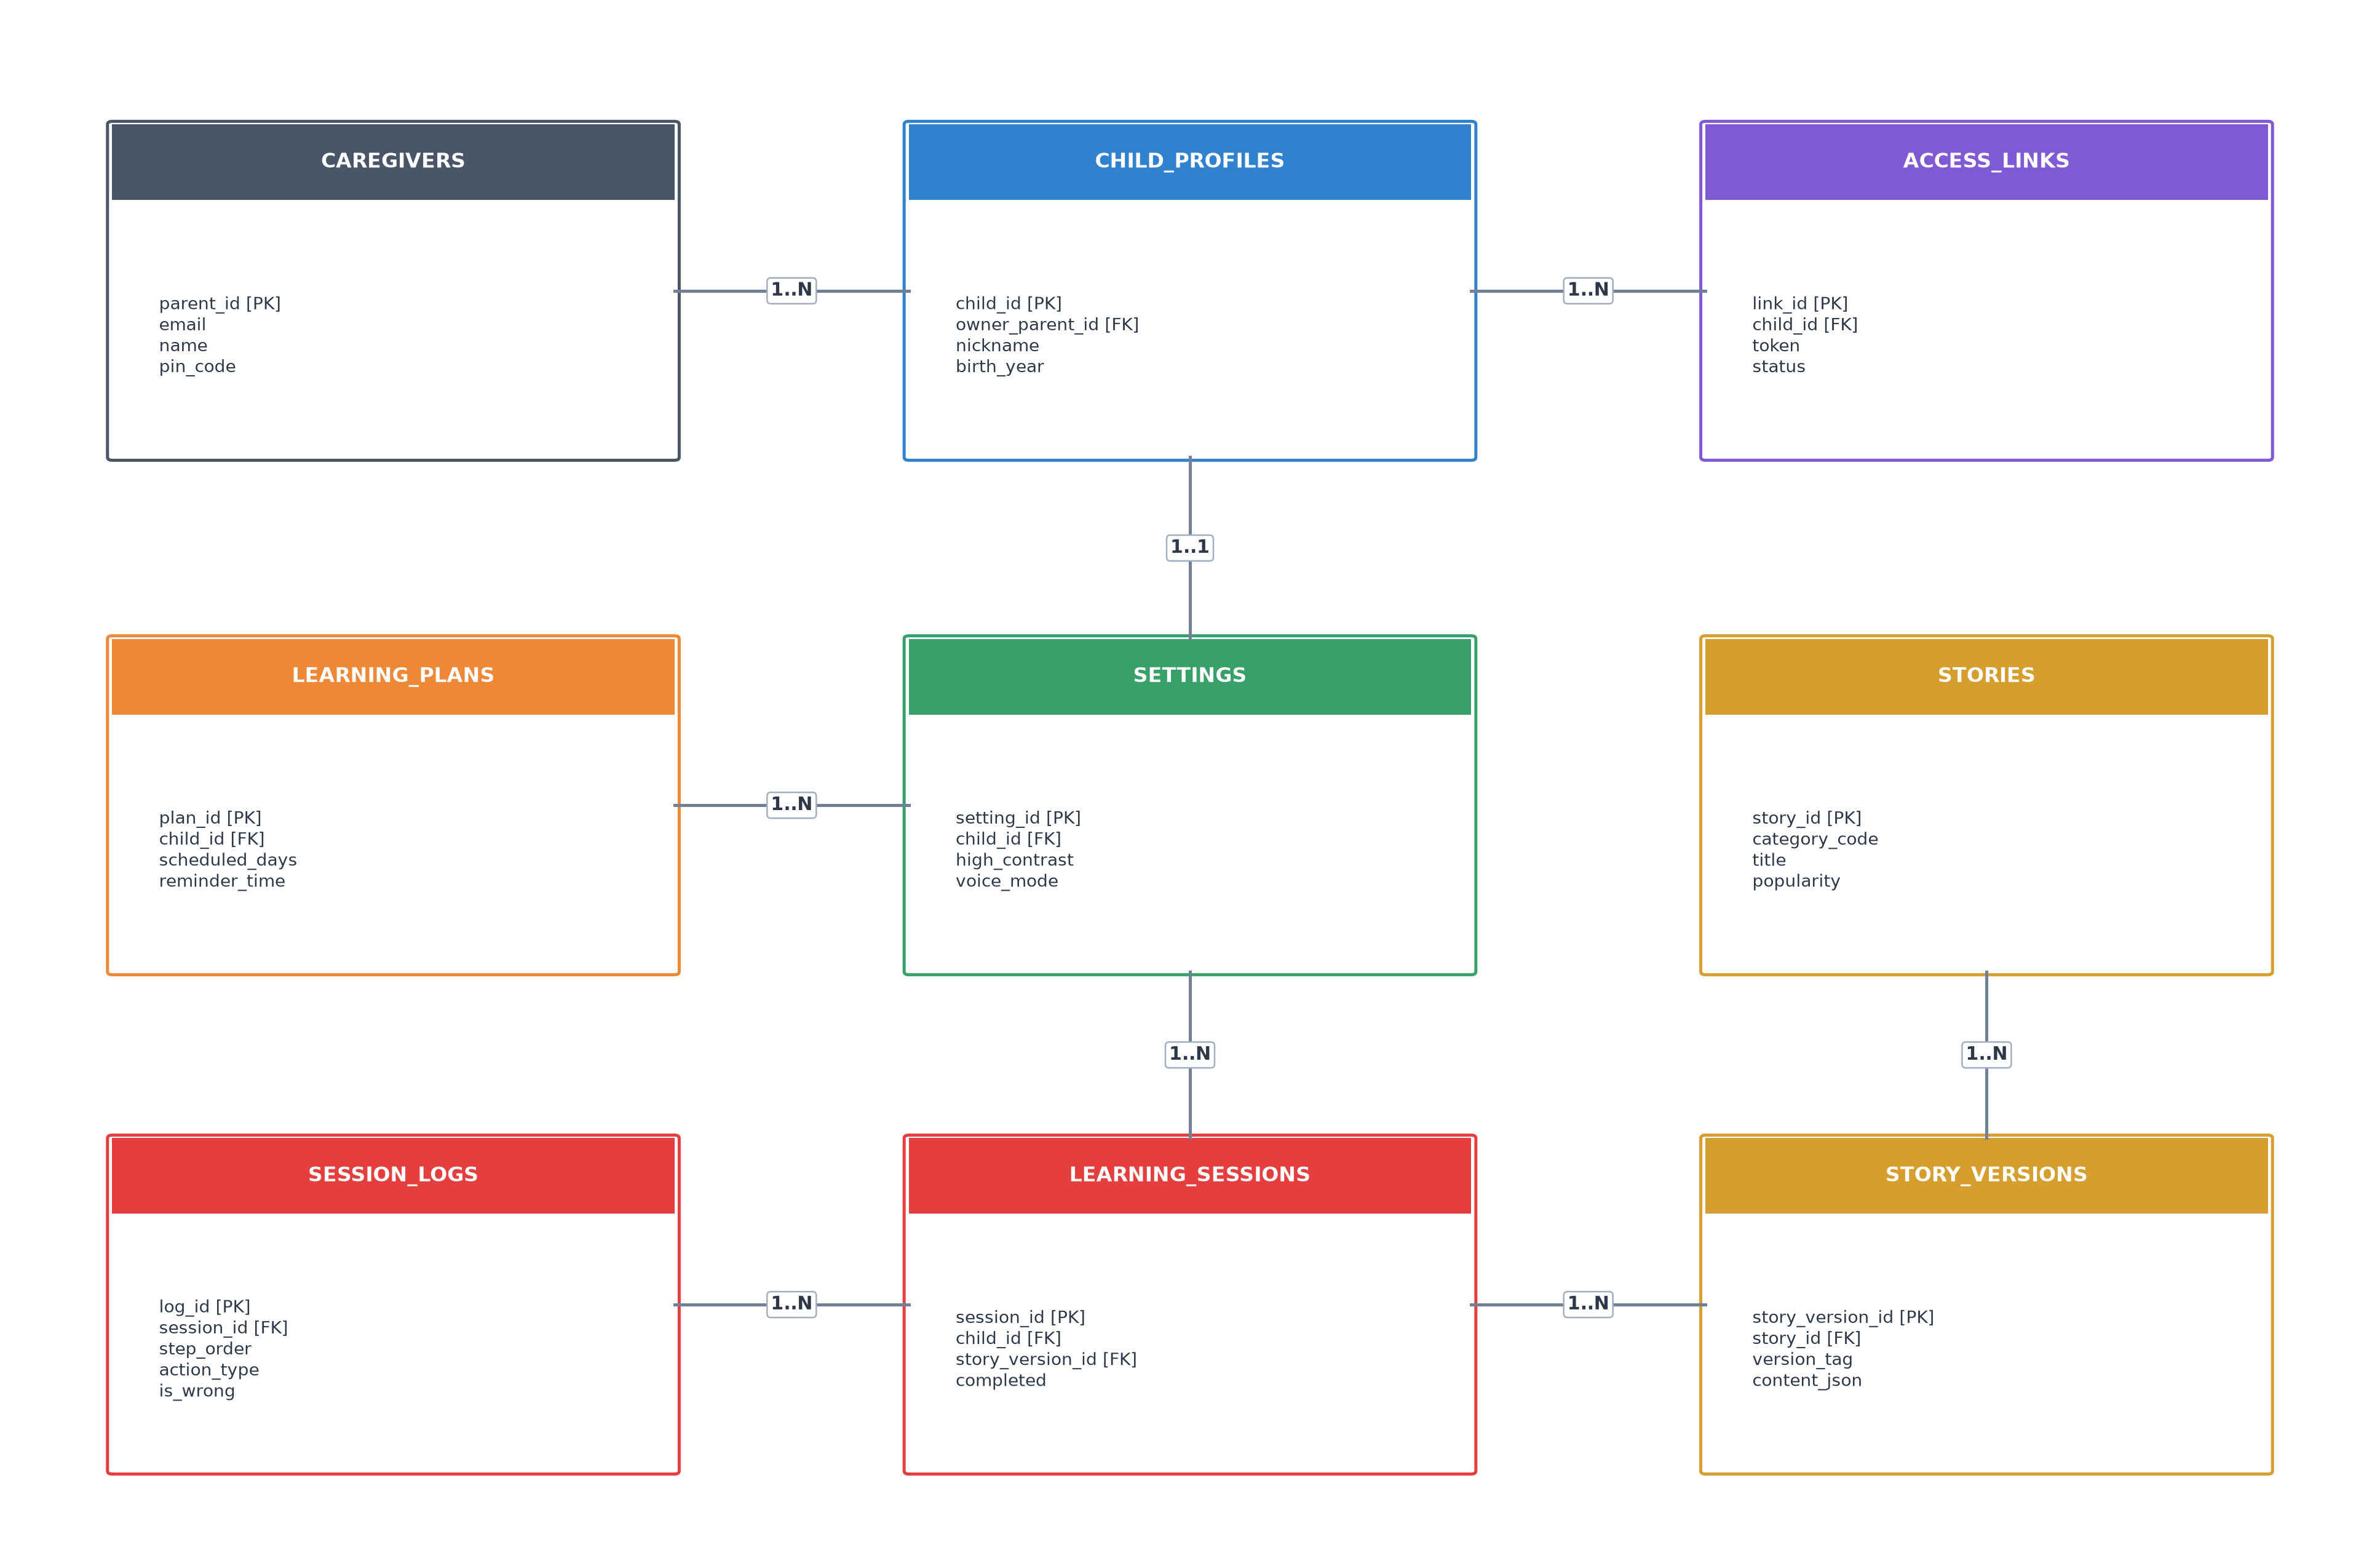
\includegraphics[width=0.95\textwidth]{figures/sqlite_erd.png}
\caption{SQLite Entity-Relationship Diagram (ERD)}
\label{fig:sqlite_erd}
\end{figure}



\subsection{Key Schema Design Decisions}


\begin{enumerate}
  \item \textbf{Separation of \texttt{STORIES} and \texttt{STORY\_VERSIONS} (\texttt{FR09}, \texttt{FR20})}:
\end{enumerate}
\begin{itemize}
  \item The \texttt{STORIES} table holds the canonical story identifier and category, whereas all scene steps, choice cards, and \texttt{why\_explanation\_text} records belong to an immutable \texttt{STORY\_VERSIONS} record.
  \item \texttt{LEARNING\_SESSIONS} references both \texttt{story\_id} and \texttt{story\_version\_id}. When a caregiver opens \texttt{Session Review} (\texttt{S16}) for a historical session, the query joins on \texttt{story\_version\_id} to render the exact wording and explanation the child saw during that session, even if the story was subsequently updated.
\end{itemize}
\begin{enumerate}
  \item \textbf{Non-Punitive Event Logging in \texttt{SESSION\_INTERACTIONS} (\texttt{DD17}, \texttt{DD18}, \texttt{DD38})}:
\end{enumerate}
\begin{itemize}
  \item \texttt{SESSION\_INTERACTIONS} intentionally omits \texttt{score} or \texttt{is\_wrong} columns. Instead, it records a chronological stream of behavioral events (\texttt{CHOOSE\_TAP}, \texttt{CHOOSE\_VOICE}, \texttt{REPLAY}, \texttt{RETRY}, \texttt{PAUSE}, \texttt{HELP}) alongside \texttt{attempt\_number}, allowing caregivers to understand how the child explored the scenario without reducing the session to a diagnostic grade.
\end{itemize}
\begin{enumerate}
  \item \textbf{Scoped Teacher Authorization via \texttt{PROFILE\_ACCESS\_LINKS} (\texttt{FR04})}:
\end{enumerate}
\begin{itemize}
  \item Every query fetching child profiles or session histories for a user with \texttt{role\_type = 'TEACHER'} enforces an \texttt{INNER JOIN} against \texttt{PROFILE\_ACCESS\_LINKS} filtered by \texttt{link\_status = 'ACTIVE'}.
\end{itemize}



\section{Sequence Diagrams and State Diagram}



\subsection{Sequence Diagram 1: Story Learning Flow and Version-Pinned Caregiver Review}


The sequence diagram below illustrates the end-to-end flow from caregiver story preview and \texttt{Child Mode} launch, through the child's \texttt{Understand} $\rightarrow$ \texttt{Predict} $\rightarrow$ \texttt{Choose} $\rightarrow$ \texttt{Observe} $\rightarrow$ \texttt{Understand Why} $\rightarrow$ \texttt{Repeat} loop, to the version-pinned caregiver review:


\begin{figure}[htbp]
\centering
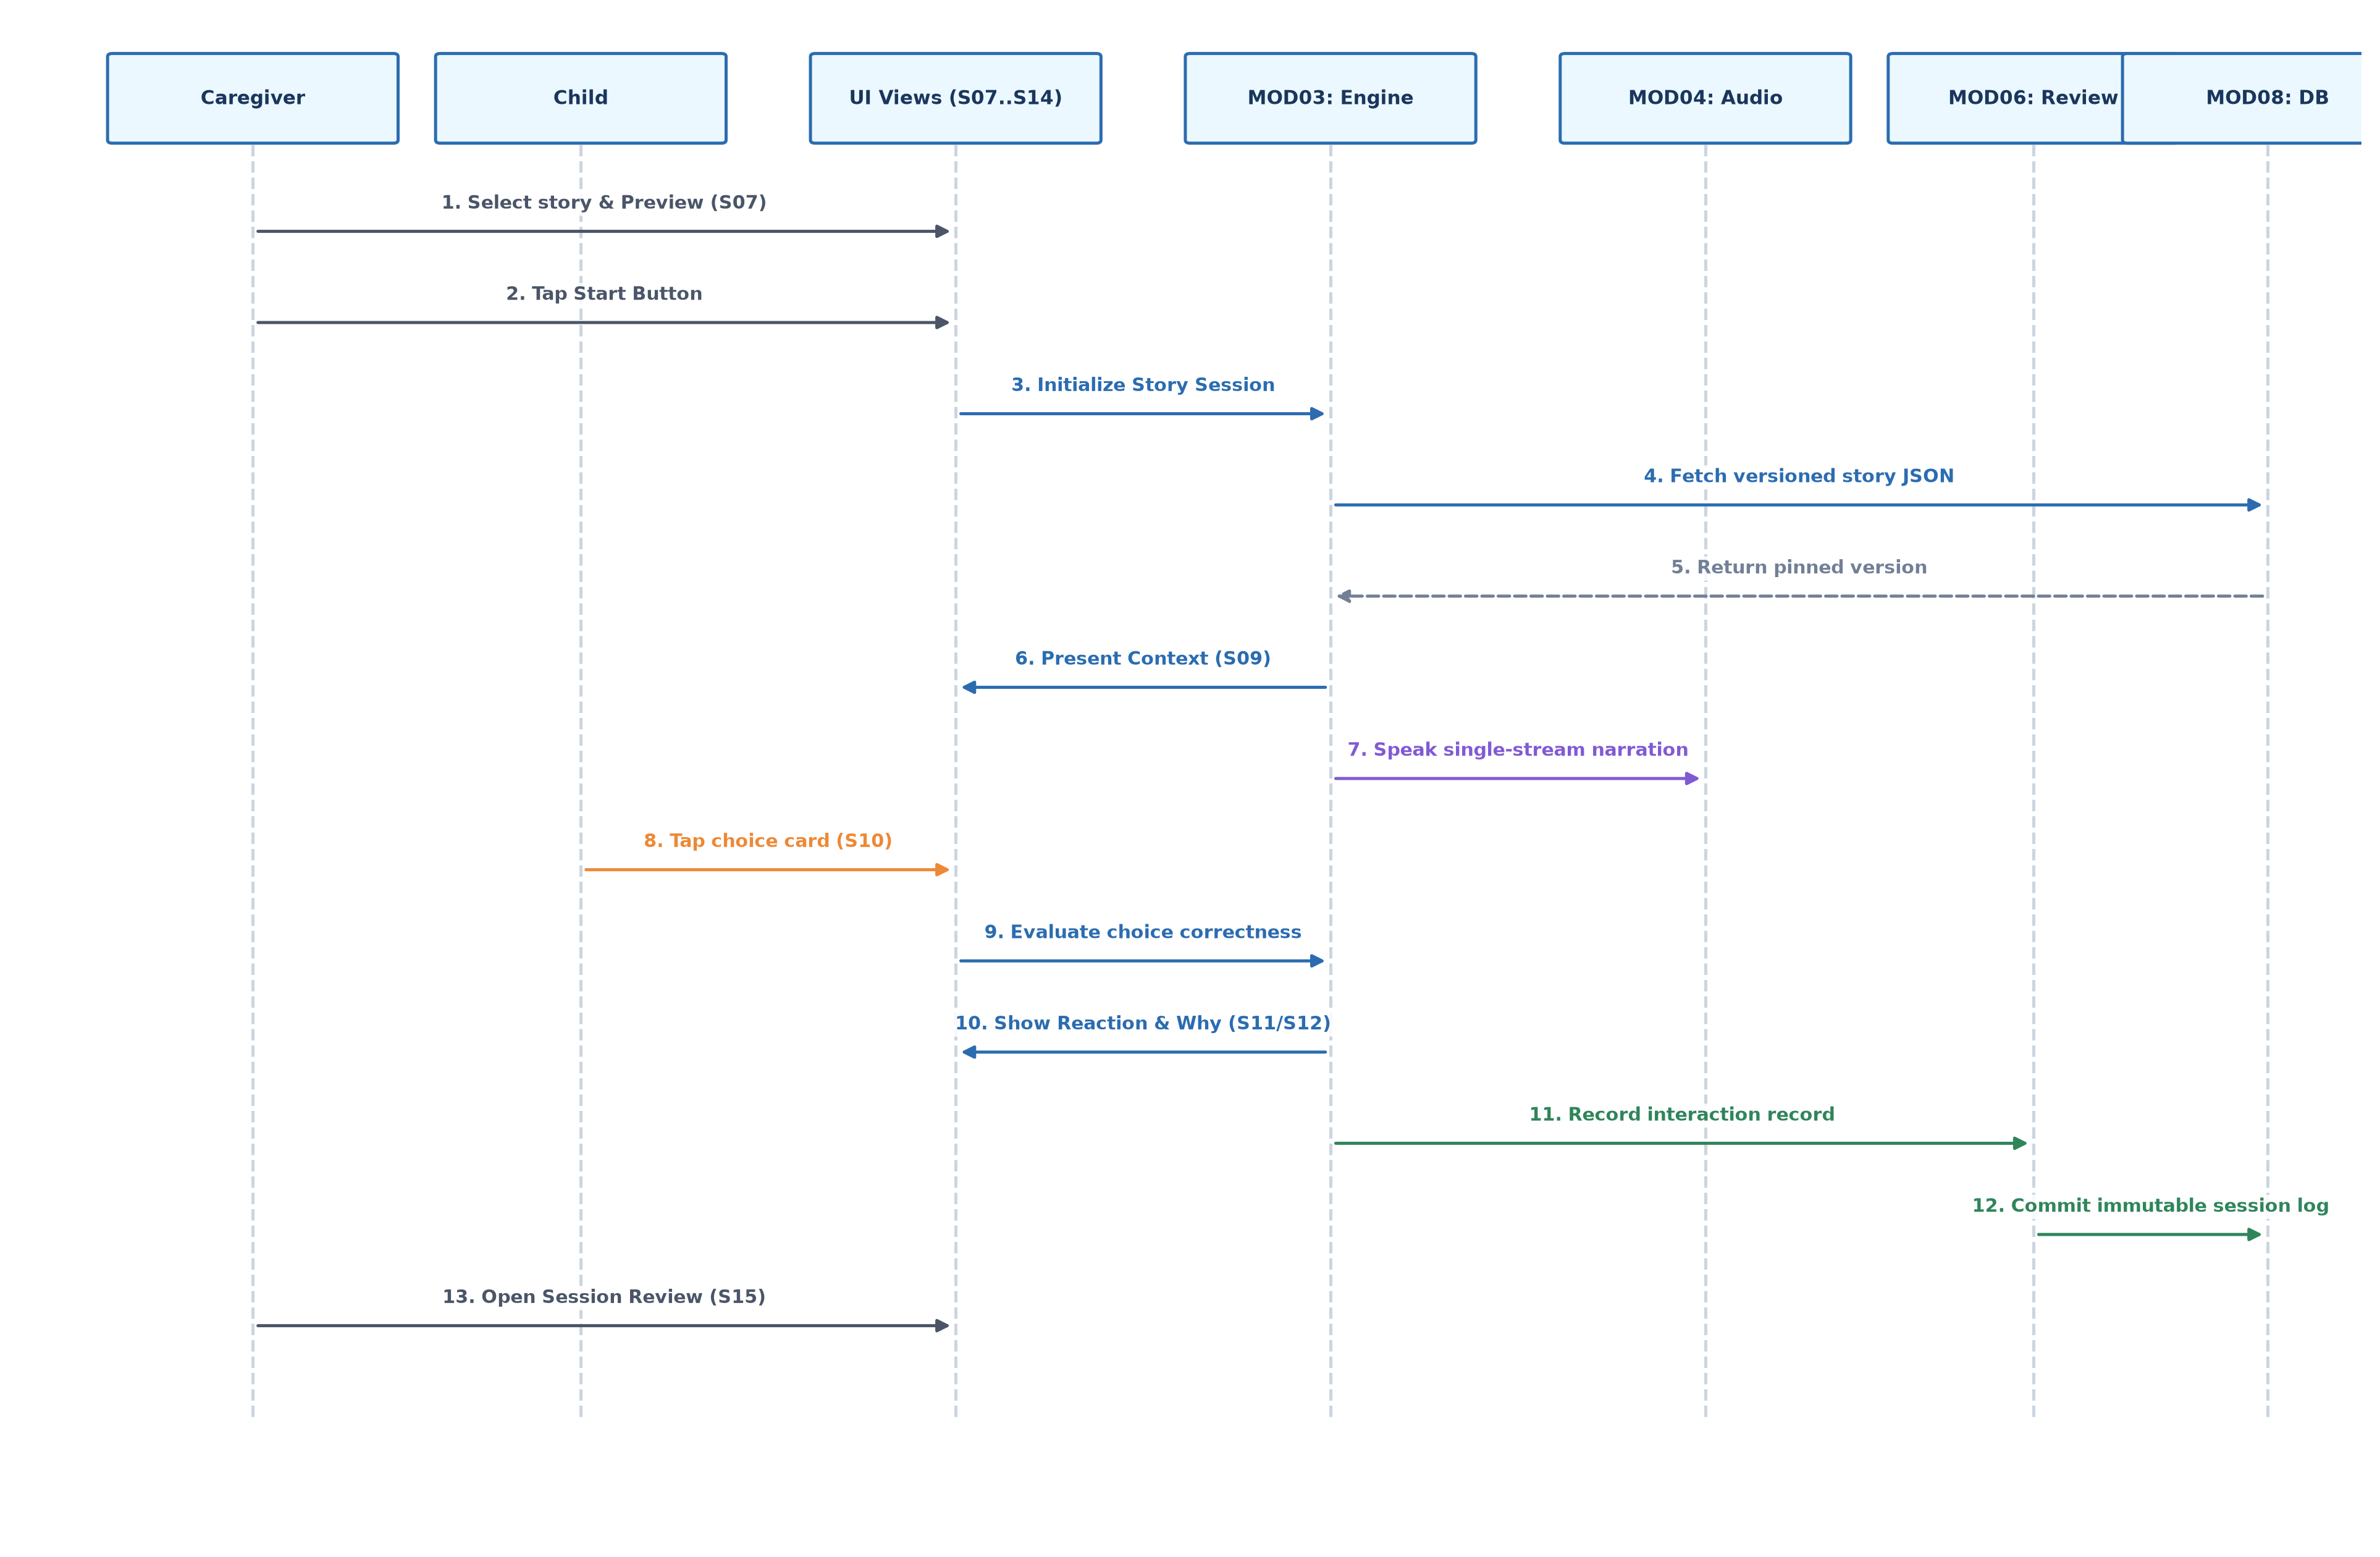
\includegraphics[width=0.95\textwidth]{figures/sequence_story_learning.png}
\caption{Sequence Diagram: Story Learning Flow and Version-Pinned Review}
\label{fig:sequence_story_learning}
\end{figure}



\subsection{Sequence Diagram 2: Scenario E Voice Interaction and Touch Fallback Flow}


The second sequence diagram models the bounded voice interaction in Scenario E (\texttt{S24}), illustrating how the child can always complete the step via touch cards if microphone access is denied or speech is not recognized:


\begin{figure}[htbp]
\centering
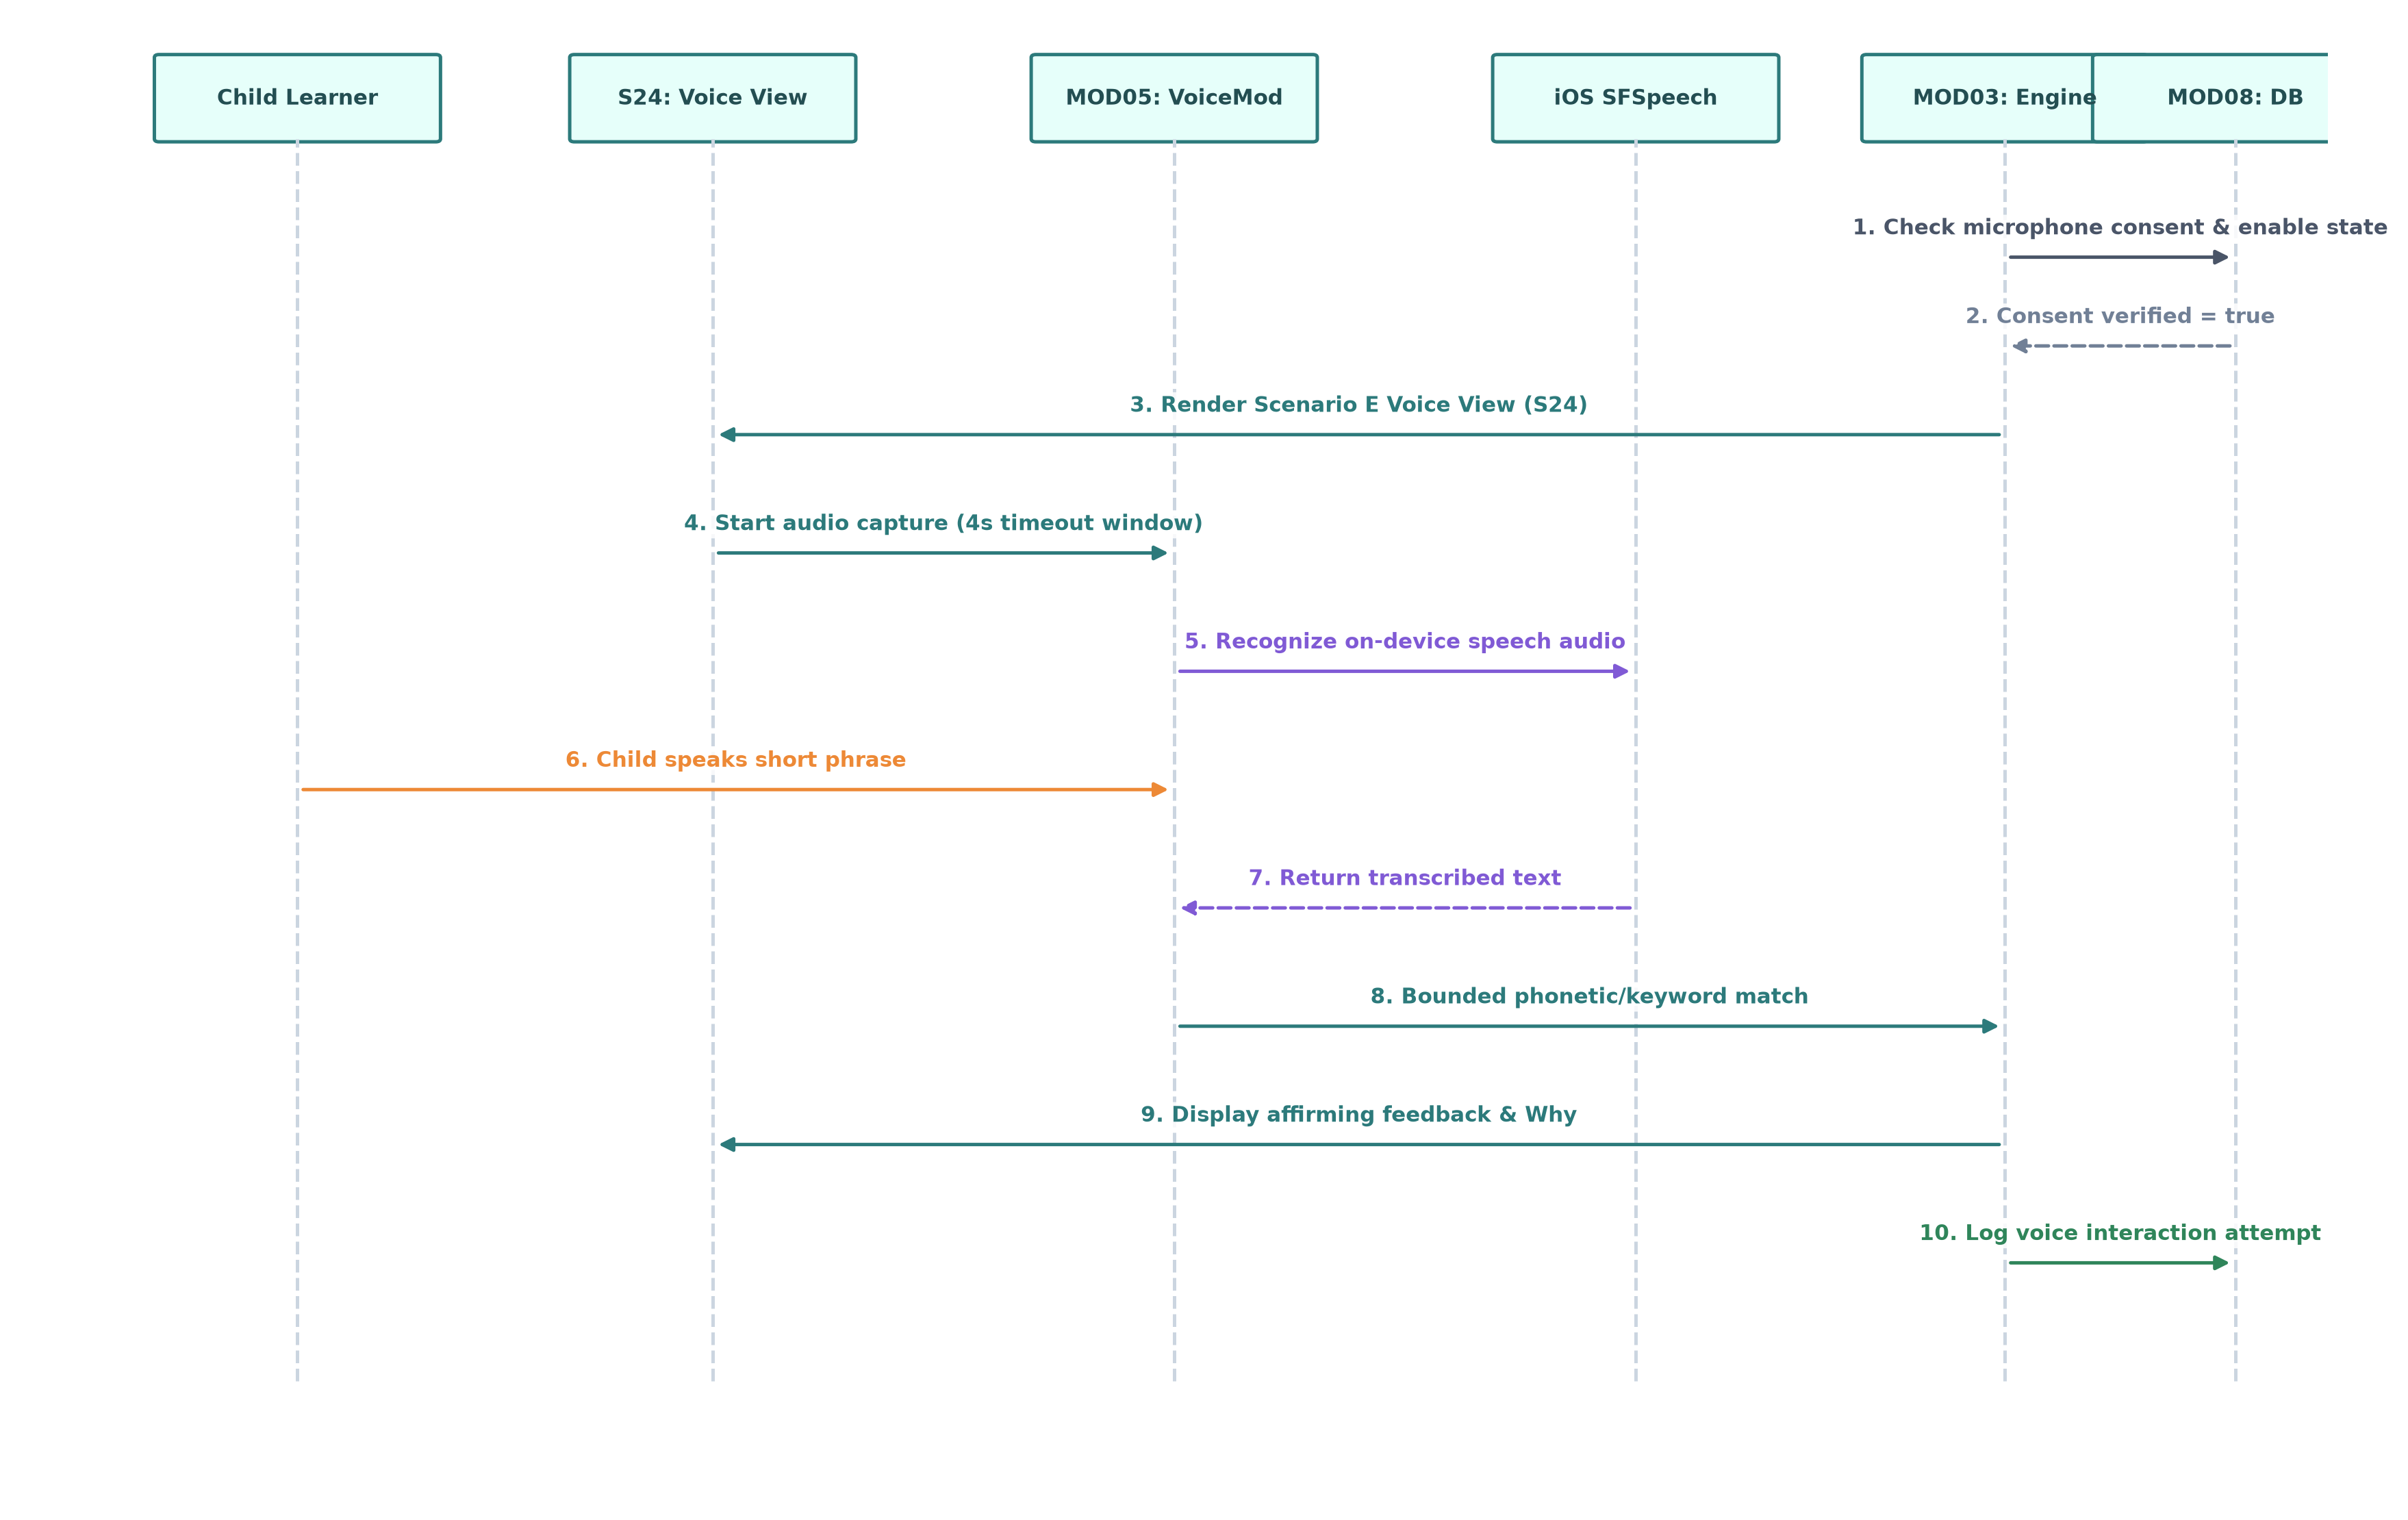
\includegraphics[width=0.95\textwidth]{figures/sequence_voice_interaction.png}
\caption{Sequence Diagram: Scenario E Voice Interaction and Touch Fallback Flow}
\label{fig:sequence_voice_interaction}
\end{figure}



\subsection{State Diagram: Story Player State Machine}


The state machine diagram below specifies the lifecycle of an interactive story session, ensuring that pausing, requesting help, or encountering an error preserves the child's context (\texttt{DD37}, \texttt{DD40}):


\begin{figure}[htbp]
\centering
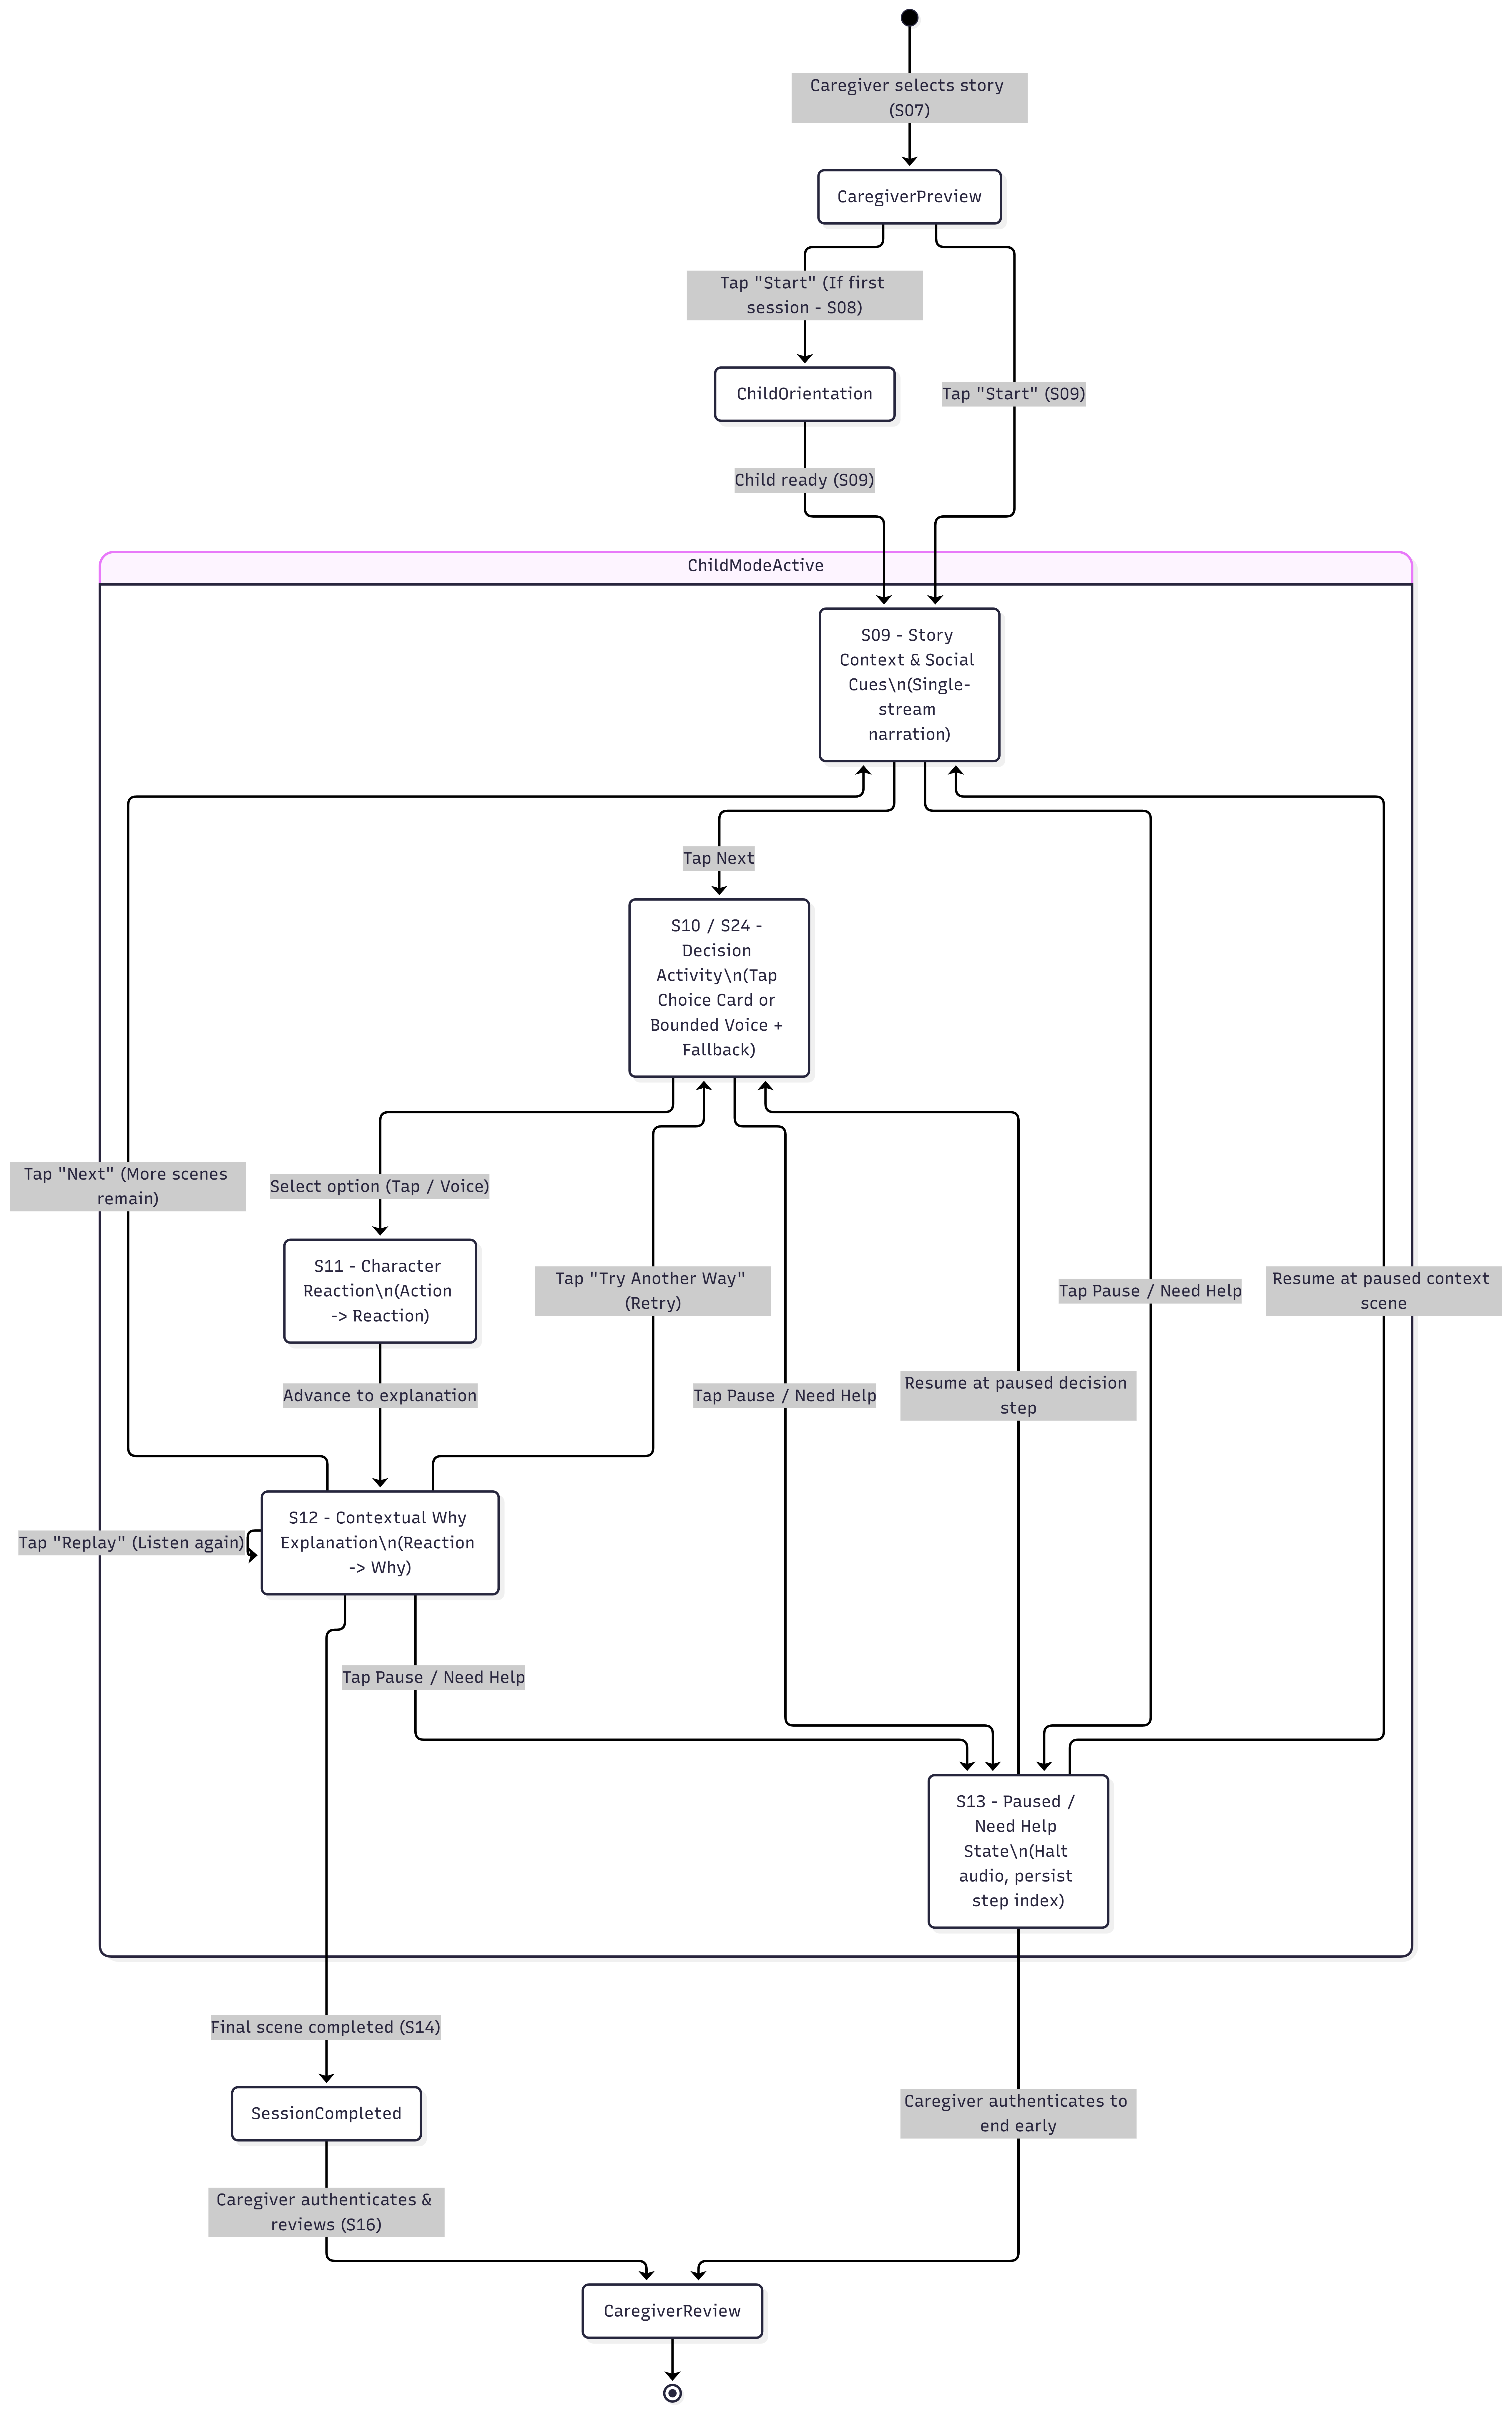
\includegraphics[width=0.95\textwidth]{figures/state_machine.png}
\caption{State Diagram: Story Player State Machine}
\label{fig:state_machine}
\end{figure}



\section{AI and Voice Interaction Design}



\subsection{Explainable Hybrid Grounded AI Recommendation for Parents (\texttt{MOD07})}


To satisfy \texttt{UN09}, \texttt{FR17}, and \texttt{DD39}, the Parent AI Suggestion feature on screen \texttt{S18} is designed around a \textbf{Hybrid Grounded Recommendation Architecture}:

\begin{enumerate}
  \item \textbf{Strict Library Grounding}: The AI module never fabricates unreviewed stories. Its input is strictly bounded to: (a) the situational goal selected or entered by the parent, (b) anonymizable recent story IDs (only if opted in on \texttt{S20}), and (c) the catalog of verified \texttt{STORIES} and \texttt{STORY\_VERSIONS} in the library.
  \item \textbf{Explainable Output Schema}: Every recommendation returned to \texttt{S18} must contain three structured fields:
\end{enumerate}
\begin{itemize}
  \item \texttt{recommended\_story\_id}: A valid story identifier existing in the local library.
  \item \texttt{match\_reason\_text}: A clear, human-readable explanation of why this story matches the parent's stated goal (e.g., \textit{"Recommended because it introduces the stethoscope sensation and practices signaling Mom when feeling nervous at the clinic"}).
  \item \texttt{alternative\_category\_code}: A related category tag allowing the parent to browse other options freely.
\end{itemize}
\begin{enumerate}
  \item \textbf{Deterministic Local Rule-Based Fallback}: When the device is offline, AI history consent is disabled, or the API exceeds the \textbf{$5\text{-second}$} timeout (\texttt{AI Timeout}), \texttt{ParentCoachService} automatically switches to local keyword and category-tag matching against SQLite so the parent always receives immediate, explainable suggestions.
\end{enumerate}



\subsection{Bounded On-Device Voice Interaction for Scenario E (\texttt{MOD05})}


\begin{itemize}
  \item \textbf{No Open-Ended Generative Voice Chat (\texttt{DD36})}: To eliminate unpredictable AI responses and expressive language pressure, Scenario E (\texttt{S24}) uses native speech recognition (\texttt{SFSpeechRecognizer} with \texttt{requiresOnDeviceRecognition} enabled where supported) strictly to match keywords against pre-authored target phrases.
  \item \textbf{Lenient Keyword Matching \& Zero Pronunciation Grading}: Detection of any core functional keyword from the model phrase (e.g., matching \textit{"play"} or \textit{"join"} for \textit{"Can I play too?"}) is accepted as a valid communicative attempt.
  \item \textbf{First-Class Parallel Touch Alternative}: Illustrated choice cards remain visible and active alongside the microphone button on \texttt{S24} at all times.
\end{itemize}



\section{Privacy and Security Design}


Bear Buddy's privacy and security architecture operationalizes \textbf{Privacy and Agency by Design (\texttt{P11})} and aligns with UNICEF's Guidance on AI and Children:

\noindent\begin{xltabular}{\textwidth}{|p{4.0cm}|X|}
\hline
\textbf{Privacy \& Security Dimension} & \textbf{Technical Implementation in Bear Buddy} \\ \hline
\endhead
\textbf{1. Data Minimization \& Ephemeral Voice Processing (\texttt{DD33}, \texttt{NFR14})} & $\bullet$ Child profiles store only a display \texttt{nickname} and functional support settings; full legal names, exact birthdates, home addresses, and clinical diagnoses are never collected. \newline $\bullet$ Microphone audio in Scenario E (\texttt{S24}) is processed exclusively in volatile RAM buffers for keyword matching and deallocated immediately after the step completes; no audio files are ever written to disk or transmitted externally. \\ \hline
\textbf{2. Protected Mode Boundary (\texttt{Caregiver Gate})} & $\bullet$ All transitions into \texttt{Caregiver Mode}, privacy settings (\texttt{S20}), session reviews (\texttt{S15}–\texttt{S16}), and external links are guarded by \texttt{CaregiverAuthGuard} using a caregiver PIN or OS biometric authentication (FaceID/TouchID), rather than trivial arithmetic prompts that children can guess (as noted in Section 5.2.1). \\ \hline
\textbf{3. Role-Based Access Control (\texttt{RBAC}: Parent vs. Teacher)} & $\bullet$ The Parent (\texttt{PERS02}) retains sole ownership (\texttt{owner\_parent\_id}) of the child profile. \newline $\bullet$ A Support Teacher (\texttt{PERS03}) can access a profile only while an \texttt{ACTIVE} record exists in \texttt{PROFILE\_ACCESS\_LINKS}. Revoking the link on \texttt{S20} immediately terminates teacher access. \\ \hline
\textbf{4. Anonymization Gateway for AI Queries (\texttt{NFR15})} & $\bullet$ Before \texttt{MOD07} dispatches any recommendation query, the \texttt{PrivacySanitizer} middleware strips \texttt{child\_id}, \texttt{nickname}, and free-text notes, transmitting only high-level situational goal tags and story IDs. \\ \hline
\textbf{5. Parental Auditability \& Right to Erasure (\texttt{FR23})} & $\bullet$ On the \texttt{Privacy and Access} screen (\texttt{S20}), parents can inspect the \texttt{CONSENT\_AUDIT\_LOGS} history, revoke microphone or AI permissions at any time, and execute immediate cascading deletion of session histories or entire child profiles from SQLite. \\ \hline
\end{xltabular}
